\let\negmedspace\undefined
\let\negthickspace\undefined
\documentclass[journal]{IEEEtran}
\usepackage[a5paper, margin=10mm, onecolumn]{geometry}
%\usepackage{lmodern} % Ensure lmodern is loaded for pdflatex
\usepackage{tfrupee} % Include tfrupee package

\setlength{\headheight}{1cm} % Set the height of the header box
\setlength{\headsep}{0mm}     % Set the distance between the header box and the top of the text

\usepackage{gvv-book}
\usepackage{gvv}
\usepackage{cite}
\usepackage{amsmath,amssymb,amsfonts,amsthm}
\usepackage{algorithmic}
\usepackage{graphicx}
\usepackage{textcomp}
\usepackage{xcolor}
\usepackage{txfonts}
\usepackage{listings}
\usepackage{enumitem}
\usepackage{mathtools}
\usepackage{gensymb}
\usepackage{comment}
\usepackage[breaklinks=true]{hyperref}
\usepackage{tkz-euclide} 
\usepackage{listings}
% \usepackage{gvv}                                        
\def\inputGnumericTable{}                                 
\usepackage[latin1]{inputenc}                                
\usepackage{color}                                            
\usepackage{array}                                            
\usepackage{longtable}                                       
\usepackage{calc}  
\usepackage{amsmath,amssymb}

\usepackage{multicol}                                         
\usepackage{hhline}                                           
\usepackage{ifthen}                                           
\usepackage{lscape}
\begin{document}

\bibliographystyle{IEEEtran}

\title{
%	\logo{
NCERT - 12.9.7.1.2

\large{EE1003}
%	}
}
\author{Homa Harshitha Vuddanti

(EE24BTECH11062)
}	

\maketitle

\bigskip

\renewcommand{\thefigure}{\theenumi}
\renewcommand{\thetable}{\theenumi}
\textbf{Question}: Find the order and degree of the differential equation $\brak{\frac{dy}{dx}}^3-4\brak{\frac{dy}{dx}}^2+7y=\sin x$\\
\textbf{Solution:} \\
The degree of a differential equation is the power of the highest derivative, provided that the equation is free from fractional or radical powers of the derivatives.\\
Order is the highest derivative that appears in the differential equation.\\
The given equation is 
\begin{align}
\brak{\frac{dy}{dx}}^3-4\brak{\frac{dy}{dx}}^2+7y=\sin x \label{eq:1}
\end{align}
Hence, the given equation has an order of 1 and degree of 3.\\
\textbf{Numeric solution:}\\
Runge Kutta method:\\
For an equation $y^\prime=f\brak{x,y}$, given $y\brak{x_0}=y_0$, the next value $y$ can be calculated as
\begin{align}
y_{n+1}&=y_n+\frac{1}{6}\brak{k_1+2k_2+2k_3+k_4}\\
x_{n+1}&=x_n+h
\end{align}
where
\begin{align}
k_1&=hf\brak{x_n,y_n}\\
k_2&=hf\brak{x_n+\frac{h}{2},y_n+\frac{k_1}{2}}\\
k_3&=hf\brak{x_n+\frac{h}{2},y_n+\frac{k_2}{2}}\\
k_4&=hf\brak{x_n+\frac{h}{2},y_n+k_3}
\end{align}
This ensures slope is evaluated at multiple points instead of just at the start. \\
Numeric solution can be obtained by assuming the initial conditions as $\brak{x_0,y_0}$ to be, say (0,0).\\
Taking $\frac{dy}{dx}=t$, we get
\begin{align}
t^3-4t^2=\sin x-7y\\
\frac{dt}{dx}=\frac{\cos x-7t}{3t^2-8t}
\end{align}
Computing $k_1,k_2,k_3$ and $k_4$ for $\brak{x_1,y_1}$
\begin{align}
k_1&=hf\brak{x_n,y_n,t_n}\\
k_2&=hf\brak{x_n+\frac{h}{2},y_n+\frac{k_1}{2},t_n+\frac{k_1}{2}}\\
k_3&=hf\brak{x_n+\frac{h}{2},y_n+\frac{k_2}{2},t_n+\frac{k_2}{2}}\\
k_4&=hf\brak{x_0+\frac{h}{2},y_n+k_3,t_n+k_3}\\
y_{n+1}&=y_n+\frac{1}{6}\brak{k_1+2k_2+2k_3+k_4}\\
t_{n+1}&=t_n+\frac{1}{6}\brak{k_1+2k_2+2k_3+k_4}
\end{align}
We take a range \sbrak{x_0,x_{end}} and at each step try to calculate k values for $y$ and $t$.
\begin{align}
k_{1y}&= ht_n\\
k_{1t}&=h\brak{\sin x_n-{t_n}^3+4{t_n}^2-7y_n}\\
k_{2y}&= h\brak{t_n+\frac{k_{1t}}{2}}\\
k_{2t}&=h\brak{\sin \brak{x_n+\frac{h}{2}}-{t_n+\frac{k_{1t}}{2}}^3+4{t_n+\frac{k_{1t}}{2}}^2-7\brak{y_n+\frac{k_{1y}}{2}}}\\
k_{3y}&= h\brak{t_n+\frac{k_{2t}}{2}}\\
k_{3t}&=h\brak{\sin \brak{x_n+\frac{h}{2}}-{t_n+\frac{k_{2t}}{2}}^3+4{t_n+\frac{k_{2t}}{2}}^2-7\brak{y_n+\frac{k_{2y}}{2}}}\\
k_{4y}&=h\brak{t_n+k_{3t}}\\
k_{4t}&=h\brak{\sin\brak{x_n+h}-\brak{v_n+k_{3t}}^3+4\brak{t_n+k_{3t}}^2-7\brak{y_n+k_{3y}}}
\end{align}
Then the next point will be of the form 
\begin{align}
y_{n+1}=y_n+\frac{1}{6}\brak{k_{1y}+2k_{2y}+2k_{3y}+k_{4y}}\\
t_{n+1}=t_n+\frac{1}{6}\brak{k_{1t}+2k_{2t}+2k_{3t}+k_{4t}}
\end{align}
we then increment $x_n$ until we reach $x_{end}$\\
\textbf{Plotting:}
By taking 
\begin{align}
\brak{x_0,y_0,t_0}&=\brak{0,0,0}\\
h&=0.1\\
x_{end}&=5
\end{align}
\begin{figure}[h!]
   \centering
   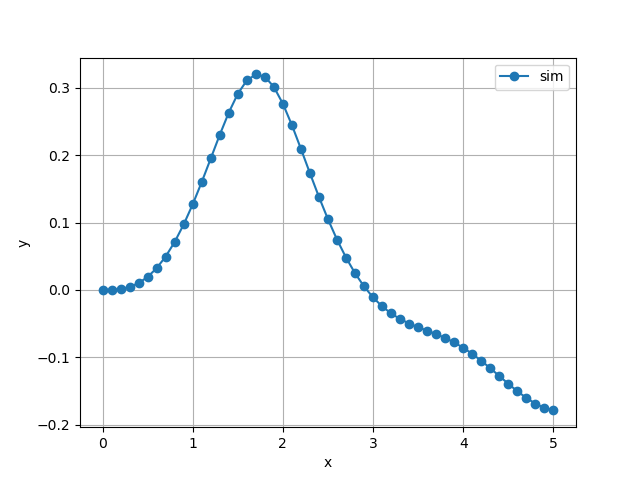
\includegraphics[width=1\columnwidth]{Figs/Figure_1.png}
   \caption{Plot}
\end{figure}
\end{document}

